\documentclass[answers]{exam}

%% Language and font encodings
\usepackage[english]{babel}
\usepackage[utf8x]{inputenc}
\usepackage[T1]{fontenc}
% \usepackage{enumitem}
%% Sets page size and margins
\usepackage[a4paper,margin=2cm]{geometry}

%% Useful packages
\usepackage{amsmath}
\usepackage{amssymb}
\usepackage{graphicx}
\usepackage{paralist}
\usepackage{framed}
\usepackage{tikz}
\usepackage{float}
\usepackage{listings}
\usepackage{xcolor}
\tikzset{
  % define the bar graph element
  bar/.pic={
    \fill (-.1,0) rectangle (.1,#1) (0,#1) node[above,scale=1/2]{$#1$};
  }
}
\definecolor{codegreen}{rgb}{0,0.6,0}
\definecolor{codegray}{rgb}{0.5,0.5,0.5}
\definecolor{codepurple}{rgb}{0.58,0,0.82}
\definecolor{backcolour}{rgb}{0.95,0.95,0.92}
% Colored Python listing from https://www.overleaf.com/learn/latex/Code_listing
\definecolor{codegreen}{rgb}{0,0.6,0}
\definecolor{codegray}{rgb}{0.5,0.5,0.5}
\definecolor{codepurple}{rgb}{0.58,0,0.82}
\definecolor{backcolour}{rgb}{0.95,0.95,0.92}
 
\lstdefinestyle{mystyle}{
    backgroundcolor=\color{backcolour},   
    commentstyle=\color{codegreen},
    keywordstyle=\color{magenta},
    numberstyle=\tiny\color{codegray},
    stringstyle=\color{codepurple},
    basicstyle=\ttfamily\footnotesize,
    breakatwhitespace=false,         
    breaklines=true,                 
    captionpos=b,                    
    keepspaces=true,                 
    numbers=left,                    
    numbersep=5pt,                  
    showspaces=false,                
    showstringspaces=false,
    showtabs=false,                  
    tabsize=2
}
\lstset{style=mystyle}

\usetikzlibrary{matrix}

\setlength\FrameSep{4pt}
\title{Probability \& Statistics\\ Project}
\author{Hana Ali Rashid, hr05940\\ Tasmiya Malik, Student ID\\ Ifrah Ilyas, Student ID}
\date{\today{}}
\begin{document}
\maketitle

% \noindent \hrulefill \\
% \textbf{Instructions:}
% \begin{itemize}
%     \item \textbf{Pairs can not be cross-section.}
% \end{itemize}

% \noindent \hrulefill

\section*{Q1: Random Walk}
\subsection*{1.1}
Function implementation in Python:
\lstinputlisting[firstline=5,lastline=13,language=python]{q1.py}
Calling the function for several iterations to get multiple expected values:
\lstinputlisting[firstline=16,lastline=33,language=python]{q1.py}
\pagebreak
Histograms produced by the above code for various combinations of $n$ and $p$:\\
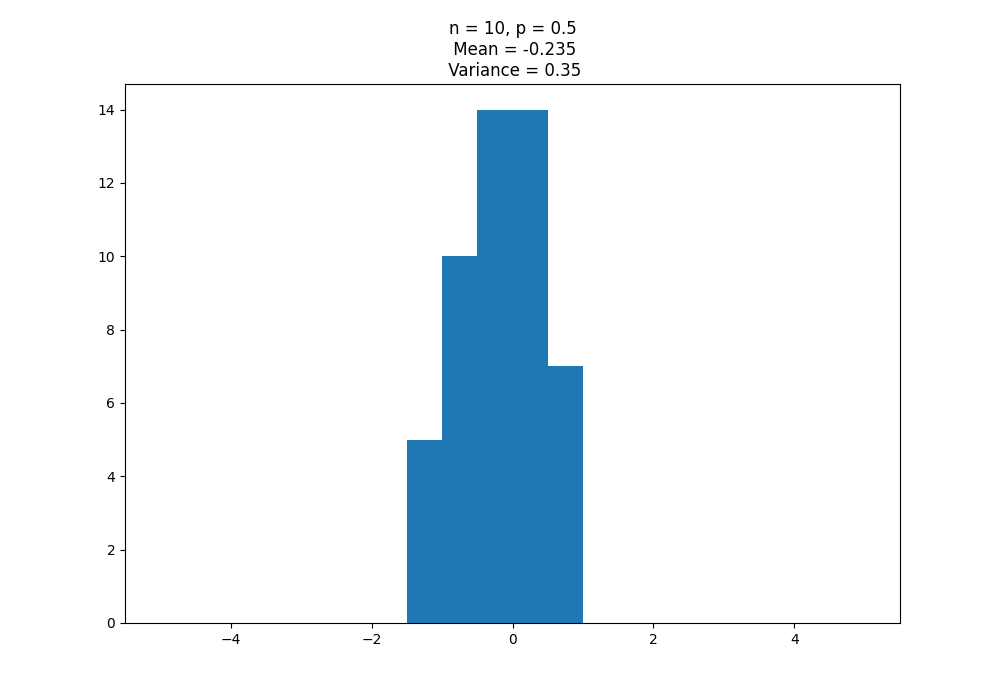
\includegraphics[scale = 0.5]{Q1_histograms/q1_n = 10_ p = 0.5.png}\\
The above histogram appears to follow a normal distribution with a mean of $3.267$ and variance of $0.233$.\\
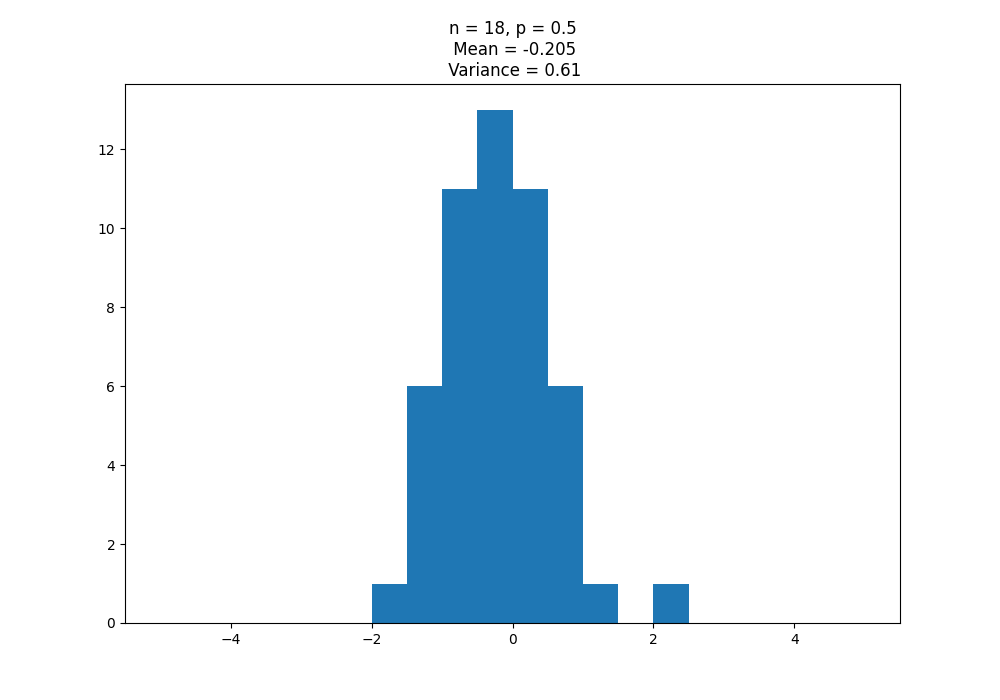
\includegraphics[scale = 0.5]{Q1_histograms/q1_n = 18_ p = 0.5.png}\\
The above histogram appears to follow a normal distribution with a mean of $3.267$ and variance of $0.233$.\\
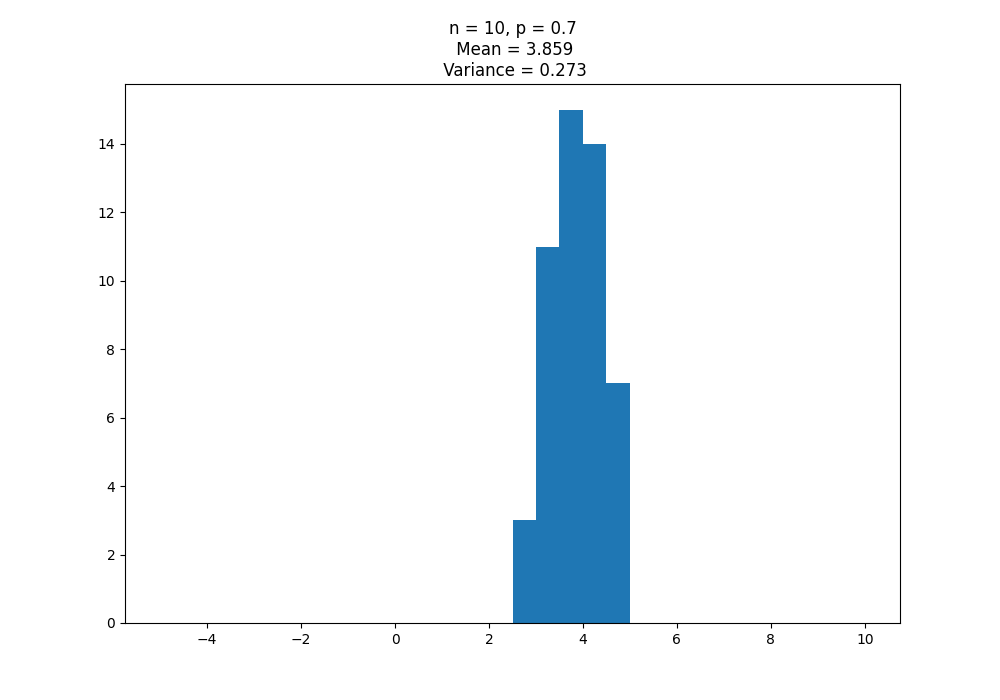
\includegraphics[scale = 0.5]{Q1_histograms/q1_n = 10_ p = 0.7.png}\\
The above histogram appears to follow a normal distribution with a mean of $3.267$ and variance of $0.233$.\\
\pagebreak
%--------------------------------  1.2  ------------------------------------
\subsection*{1.2}
Function implementation in Python:
\lstinputlisting[firstline=36,lastline=44,language=python]{q1.py}
Calling the function for several iterations to get multiple expected values:
\lstinputlisting[firstline=46,lastline=63,language=python]{q1.py}
\pagebreak
Histograms produced by the above code for various combinations of $n$ and $p$:\\
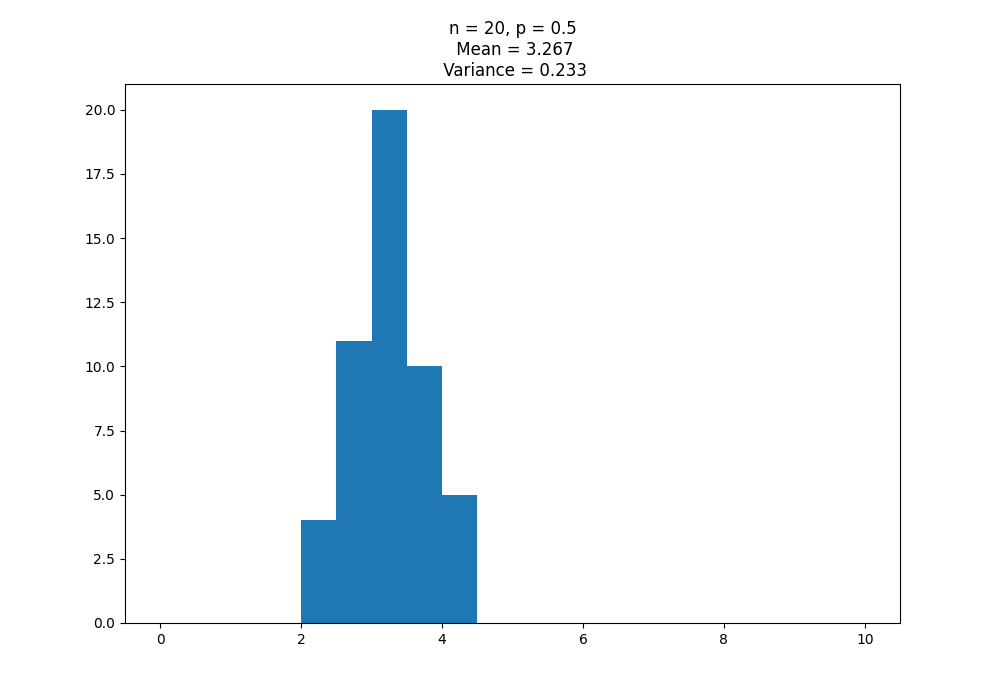
\includegraphics[scale = 0.5]{Q1_histograms/Q1.2 _n = 20_p = 0.5.png}\\
The above histogram appears to follow a normal distribution with a mean of $3.267$ and variance of $0.233$.\\
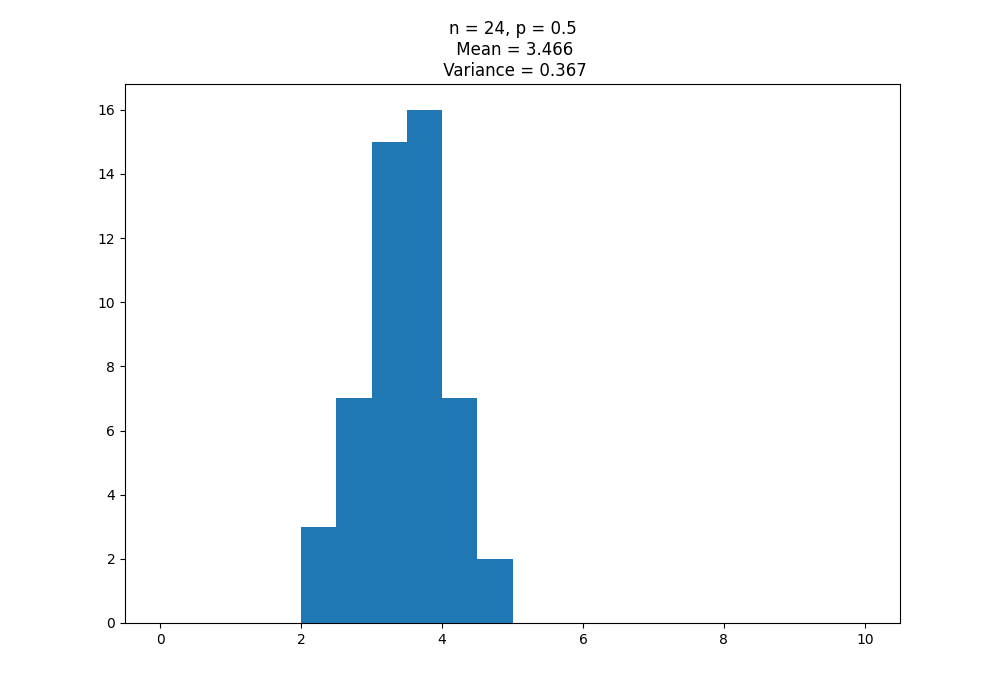
\includegraphics[scale = 0.5]{Q1_histograms/Q1.2 _n = 24_p = 0.5.png}\\
The above histogram shows that...\\
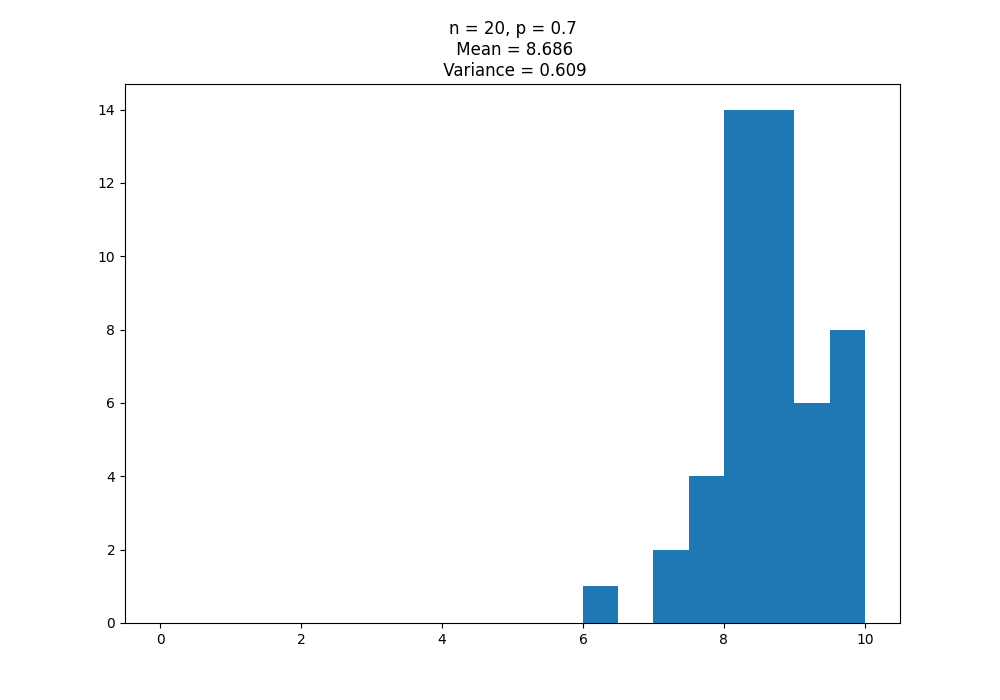
\includegraphics[scale = 0.5]{Q1_histograms/Q1.2 _n = 20_p = 0.7.png}\\
The above histogram shows that...\\
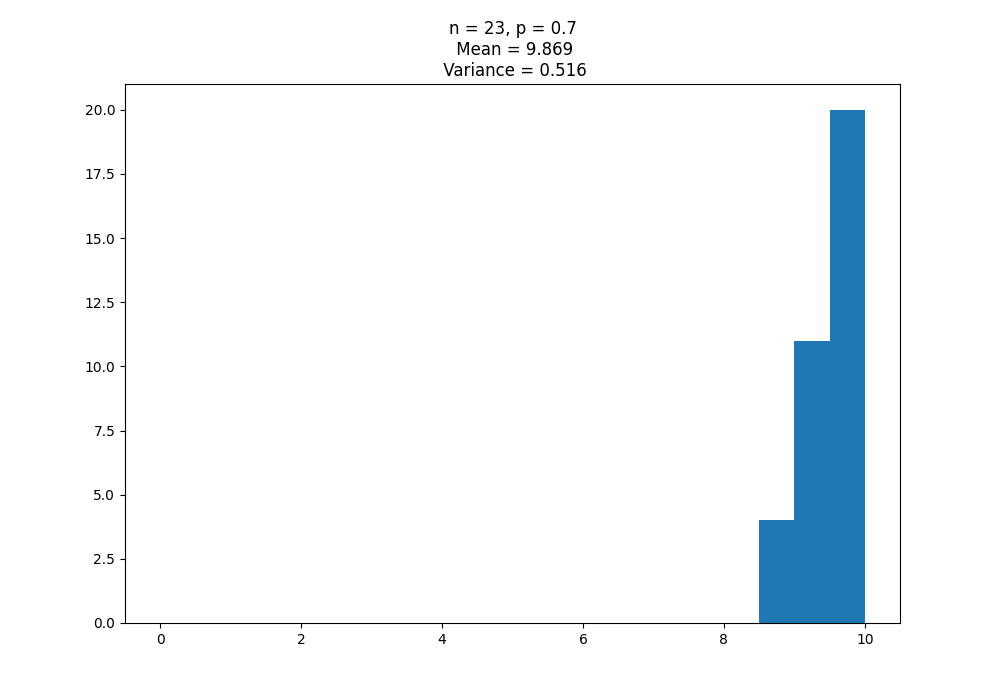
\includegraphics[scale = 0.5]{Q1_histograms/Q1.2 _n = 23_p = 0.7.png}

\pagebreak
%--------------------------------  1.3  ------------------------------------
\subsection*{1.3}
Function implementation in Python:
\lstinputlisting[firstline=65,lastline=79,language=python]{q1.py}
Calling the function for several iterations to get multiple expected values:
\lstinputlisting[firstline=81,lastline=104,language=python]{q1.py}

\end{document}